\documentclass[a4paper]{amsart}
\usepackage[utf8]{inputenc}
\usepackage{fullpage}

\usepackage[dvipsnames]{xcolor}
\usepackage{amsmath}
\usepackage{amssymb}
\usepackage{amsfonts}
\usepackage{amsthm}
\usepackage{graphicx}
\usepackage{tikz}
\usepackage{tikz-cd}
\usetikzlibrary{calc}
\usepackage{amscd}


\newtheorem{definition}{Definition}[section]
\newtheorem{theorem}{Theorem}[section]
\newtheorem{lemma}[theorem]{Lemma}
\newtheorem{remark}[theorem]{Remark}
\newtheorem{example}[theorem]{Example}
\newtheorem{proposition}[theorem]{Proposition}

\makeatletter
\newcommand\suchthat{%
 \@ifstar
  {\mathrel{}\middle|\mathrel{}}
  {\mid}%
}
\makeatother

\newcommand{\Ceins}[1]{C_{1,#1}}
\newcommand{\Czwei}[1]{C_{2,#1}}
\newcommand{\Cdrei}[1]{C_{3,#1}}
\newcommand{\Cvier}[2]{C_{4,#1,#2}}
\newcommand{\Cfive}[2]{C_{5,#1,#2}}
% \newcommand{\Ceins}{\sqrt{n}}
% \newcommand{\Czwei}{\sqrt{2n}}



\newcommand{\Perm}{{\operatorname{Perm}}}

\newcommand{\linhull}{{\operatorname{span}}}
\newcommand{\convexhull}{{\operatorname{convex}}}

\newcommand{\Poinc}{\frakP}
\newcommand{\Bogov}{\frakB}

\newcommand{\mollifier}{\frakm}

\newcommand{\eps}{\epsilon}

\newcommand{\Id}{\rm{Id}}

\newcommand{\Lip}{\rm{Lip}}

\newcommand{\diff}{\mathop{}\!\mathrm{d}}

\DeclareMathOperator{\adj}{adj}
%\newcommand{\adj}{{\rm adj}}
\newcommand{\inv}{{-1}}
\newcommand{\invt}{{-t}}
\newcommand{\tinv}{{-t}}
\newcommand{\determinant}{{\operatorname{det}}}
\DeclareMathOperator{\Jacobian}{{\rm Jac}}
% \newcommand{\Jacobian}{{\rm Jac}}
\newcommand{\dimension}{\operatorname{dim}}
\newcommand{\sgn}{\operatorname{sgn}}
\newcommand{\adjugate}{\operatorname{adj}}
\newcommand{\sym}{\operatorname{sym}}
\newcommand{\signum}{\operatorname{sgn}}
\newcommand{\kronecker}{{\hat\delta}}
\newcommand{\dom}{\operatorname{dom}}
\newcommand{\codom}{\operatorname{codom}}
\newcommand{\rng}{\operatorname{ran}}
\newcommand{\convex}{\operatorname{convex}}
\newcommand{\coker}{\operatorname{coker}}
\newcommand{\coran}{\operatorname{coran}}

\newcommand{\dif}{{\mathrm d}}
\newcommand{\Dif}{{\mathrm D}}
\newcommand{\grad}{\operatorname{grad}}
\newcommand{\Grad}{\operatorname{Grad}}
\newcommand{\curl}{\operatorname{curl}}
\newcommand{\Curl}{\operatorname{Curl}}
\newcommand{\rot}{\curl}
\newcommand{\divergence}{\operatorname{div}}
\newcommand{\diver}{\operatorname{div}}
\newcommand{\svcurl}{\operatorname{sv-curl}}
\newcommand{\vscurl}{\operatorname{vs-curl}}
\newcommand{\sdiver}{\operatorname{sdiv}}
\newcommand{\Sdiver}{\operatorname{Sdiv}}
\newcommand{\sgrad}{\operatorname{sgrad}}
\newcommand{\Sgrad}{\operatorname{Sgrad}}
\newcommand{\Laplace}{\bigtriangleup}
\newcommand{\laplace}{\bigtriangleup}
\newcommand{\laplacian}{\laplace}
\newcommand{\Laplacian}{\laplace}
% \newcommand{\cartan}{{\mathsf d}}
% \newcommand{\cartanx}{{\mathsf d}x}
\newcommand{\cartan}{d}
\newcommand{\cartanx}{dx}

%\newcommand{\argmin}{\operatorname{argmin}}
\DeclareMathOperator*{\argmin}{{\rm argmin}}

% \DeclareMathOperator*{\carapace}{{\rm corona}}
\DeclareMathOperator*{\carapace}{{\partial \rm st}}

\newcommand{\supp}{\operatorname{supp}}
\newcommand{\esssup}{{\operatorname{esssup}}}
\newcommand{\essinf}{{\operatorname{essinf}}}

\newcommand{\equivalent}{ \Longleftrightarrow }
\newcommand{\vol}{\operatorname{vol}}
\newcommand{\st}{ \mid }
\newcommand{\diam}{{\operatorname{diam}}}
\newcommand{\height}{\operatorname{height}}
\newcommand{\dist}{\operatorname{dist}}
\newcommand{\patch}{\operatorname{st}}

\newcommand{\Trace}{\operatorname{Tr}}
\newcommand{\Tr}{\operatorname{Tr}}
\newcommand{\trace}{\operatorname{tr}}
\newcommand{\normaltrace}{\operatorname{nm}}
\newcommand{\tr}{\operatorname{tr}}
\newcommand{\Ext}{\operatorname{Ext}}
\newcommand{\Ex}{\operatorname{Ex}}
\newcommand{\ext}{\operatorname{ext}}

\newcommand{\Poincare}{\sfP}
\newcommand*{\volsphere}[1]{\color{red}{S_{#1}}}
\newcommand*{\volball}[1]{B_{#1}}

\newcommand{\subsimplex}{\calS^{\downarrow}}
\newcommand{\supsimplex}{\calS^{\uparrow}}
\newcommand{\supersimplex}{\supsimplex}
\newcommand{\orientation}{\mathscr{O}}
\newcommand{\restrict}{R}

\newcommand{\Mesh}{\calT}
\newcommand{\Vertices}{\calV}
\newcommand{\Edges}{\calE}
\newcommand{\Faces}{\calF}
\newcommand{\Ball}{\calB}
\newcommand{\Sphere}{S}
\newcommand{\underlying}[1]{\left| #1 \right|}

\newcommand{\Distr}{\calD}
\newcommand{\Cont}{\calC}
\newcommand{\Lebesgue}{L}
\newcommand{\Sobolev}{W}
\newcommand{\SOBOLEV}{\bfW}
\newcommand{\SobolevLambda}{W\Lambda}
\newcommand{\Alt}{\Lambda}
\newcommand{\loc}{\rm{loc}}

\newcommand{\Ned}{{\calN d}}
\newcommand{\RT}{{\calR T}}
\newcommand{\BDM}{{\calB \calD \calM}}
  

\newcommand*{\ConstantPF}{C_{\rm{PF}}}







\newcommand{\bbA}{{\mathbb A}}
\newcommand{\bbB}{{\mathbb B}}
\newcommand{\bbC}{{\mathbb C}}
\newcommand{\bbD}{{\mathbb D}}
\newcommand{\bbE}{{\mathbb E}}
\newcommand{\bbF}{{\mathbb F}}
\newcommand{\bbG}{{\mathbb G}}
\newcommand{\bbH}{{\mathbb H}}
\newcommand{\bbI}{{\mathbb I}}
\newcommand{\bbJ}{{\mathbb J}}
\newcommand{\bbK}{{\mathbb K}}
\newcommand{\bbL}{{\mathbb L}}
\newcommand{\bbM}{{\mathbb M}}
\newcommand{\bbN}{{\mathbb N}}
\newcommand{\bbO}{{\mathbb O}}
\newcommand{\bbP}{{\mathbb P}}
\newcommand{\bbQ}{{\mathbb Q}}
\newcommand{\bbR}{{\mathbb R}}
\newcommand{\bbS}{{\mathbb S}}
\newcommand{\bbT}{{\mathbb T}}
\newcommand{\bbU}{{\mathbb U}}
\newcommand{\bbV}{{\mathbb V}}
\newcommand{\bbW}{{\mathbb W}}
\newcommand{\bbX}{{\mathbb X}}
\newcommand{\bbY}{{\mathbb Y}}
\newcommand{\bbZ}{{\mathbb Z}}

\newcommand{\bfA}{{\mathbf A}}
\newcommand{\bfB}{{\mathbf B}}
\newcommand{\bfC}{{\mathbf C}}
\newcommand{\bfD}{{\mathbf D}}
\newcommand{\bfE}{{\mathbf E}}
\newcommand{\bfF}{{\mathbf F}}
\newcommand{\bfG}{{\mathbf G}}
\newcommand{\bfH}{{\mathbf H}}
\newcommand{\bfI}{{\mathbf I}}
\newcommand{\bfJ}{{\mathbf J}}
\newcommand{\bfK}{{\mathbf K}}
\newcommand{\bfL}{{\mathbf L}}
\newcommand{\bfM}{{\mathbf M}}
\newcommand{\bfN}{{\mathbf N}}
\newcommand{\bfO}{{\mathbf O}}
\newcommand{\bfP}{{\mathbf P}}
\newcommand{\bfQ}{{\mathbf Q}}
\newcommand{\bfR}{{\mathbf R}}
\newcommand{\bfS}{{\mathbf S}}
\newcommand{\bfT}{{\mathbf T}}
\newcommand{\bfU}{{\mathbf U}}
\newcommand{\bfV}{{\mathbf V}}
\newcommand{\bfW}{{\mathbf W}}
\newcommand{\bfX}{{\mathbf X}}
\newcommand{\bfY}{{\mathbf Y}}
\newcommand{\bfZ}{{\mathbf Z}}

\newcommand{\bfa}{{\mathbf a}}
\newcommand{\bfb}{{\mathbf b}}
\newcommand{\bfc}{{\mathbf c}}
\newcommand{\bfd}{{\mathbf d}}
\newcommand{\bfe}{{\mathbf e}}
\newcommand{\bff}{{\mathbf f}}
\newcommand{\bfg}{{\mathbf g}}
\newcommand{\bfh}{{\mathbf h}}
\newcommand{\bfi}{{\mathbf i}}
\newcommand{\bfj}{{\mathbf j}}
\newcommand{\bfk}{{\mathbf k}}
\newcommand{\bfl}{{\mathbf l}}
\newcommand{\bfm}{{\mathbf m}}
\newcommand{\bfn}{{\mathbf n}}
\newcommand{\bfo}{{\mathbf o}}
\newcommand{\bfp}{{\mathbf p}}
\newcommand{\bfq}{{\mathbf q}}
\newcommand{\bfr}{{\mathbf r}}
\newcommand{\bfs}{{\mathbf s}}
\newcommand{\bft}{{\mathbf t}}
\newcommand{\bfu}{{\mathbf u}}
\newcommand{\bfv}{{\mathbf v}}
\newcommand{\bfw}{{\mathbf w}}
\newcommand{\bfx}{{\mathbf x}}
\newcommand{\bfy}{{\mathbf y}}
\newcommand{\bfz}{{\mathbf z}}


\newcommand{\calA}{{\mathcal A}}
\newcommand{\calB}{{\mathcal B}}
\newcommand{\calC}{{\mathcal C}}
\newcommand{\calD}{{\mathcal D}}
\newcommand{\calE}{{\mathcal E}}
\newcommand{\calF}{{\mathcal F}}
\newcommand{\calG}{{\mathcal G}}
\newcommand{\calH}{{\mathcal H}}
\newcommand{\calI}{{\mathcal I}}
\newcommand{\calJ}{{\mathcal J}}
\newcommand{\calK}{{\mathcal K}}
\newcommand{\calL}{{\mathcal L}}
\newcommand{\calM}{{\mathcal M}}
\newcommand{\calN}{{\mathcal N}}
\newcommand{\calO}{{\mathcal O}}
\newcommand{\calP}{{\mathcal P}}
\newcommand{\calQ}{{\mathcal Q}}
\newcommand{\calR}{{\mathcal R}}
\newcommand{\calS}{{\mathcal S}}
\newcommand{\calT}{{\mathcal T}}
\newcommand{\calU}{{\mathcal U}}
\newcommand{\calV}{{\mathcal V}}
\newcommand{\calW}{{\mathcal W}}
\newcommand{\calX}{{\mathcal X}}
\newcommand{\calY}{{\mathcal Y}}
\newcommand{\calZ}{{\mathcal Z}}

\newcommand{\fraka}{{\mathfrak a}}
\newcommand{\frakb}{{\mathfrak b}}
\newcommand{\frakc}{{\mathfrak c}}
\newcommand{\frakd}{{\mathfrak d}}
\newcommand{\frake}{{\mathfrak e}}
\newcommand{\frakf}{{\mathfrak f}}
\newcommand{\frakg}{{\mathfrak g}}
\newcommand{\frakh}{{\mathfrak h}}
\newcommand{\fraki}{{\mathfrak i}}
\newcommand{\frakj}{{\mathfrak j}}
\newcommand{\frakk}{{\mathfrak k}}
\newcommand{\frakl}{{\mathfrak l}}
\newcommand{\frakm}{{\mathfrak m}}
\newcommand{\frakn}{{\mathfrak n}}
\newcommand{\frako}{{\mathfrak o}}
\newcommand{\frakp}{{\mathfrak p}}
\newcommand{\frakq}{{\mathfrak q}}
\newcommand{\frakr}{{\mathfrak r}}
\newcommand{\fraks}{{\mathfrak s}}
\newcommand{\frakt}{{\mathfrak t}}
\newcommand{\fraku}{{\mathfrak u}}
\newcommand{\frakv}{{\mathfrak v}}
\newcommand{\frakw}{{\mathfrak w}}
\newcommand{\frakx}{{\mathfrak x}}
\newcommand{\fraky}{{\mathfrak y}}
\newcommand{\frakz}{{\mathfrak z}}
\newcommand{\frakA}{{\mathfrak A}}
\newcommand{\frakB}{{\mathfrak B}}
\newcommand{\frakC}{{\mathfrak C}}
\newcommand{\frakD}{{\mathfrak D}}
\newcommand{\frakE}{{\mathfrak E}}
\newcommand{\frakF}{{\mathfrak F}}
\newcommand{\frakG}{{\mathfrak G}}
\newcommand{\frakH}{{\mathfrak H}}
\newcommand{\frakI}{{\mathfrak I}}
\newcommand{\frakJ}{{\mathfrak J}}
\newcommand{\frakK}{{\mathfrak K}}
\newcommand{\frakL}{{\mathfrak L}}
\newcommand{\frakM}{{\mathfrak M}}
\newcommand{\frakN}{{\mathfrak N}}
\newcommand{\frakO}{{\mathfrak O}}
\newcommand{\frakP}{{\mathfrak P}}
\newcommand{\frakQ}{{\mathfrak Q}}
\newcommand{\frakR}{{\mathfrak R}}
\newcommand{\frakS}{{\mathfrak S}}
\newcommand{\frakT}{{\mathfrak T}}
\newcommand{\frakU}{{\mathfrak U}}
\newcommand{\frakV}{{\mathfrak V}}
\newcommand{\frakW}{{\mathfrak W}}
\newcommand{\frakX}{{\mathfrak X}}
\newcommand{\frakY}{{\mathfrak Y}}
\newcommand{\frakZ}{{\mathfrak Z}}







\newcommand{\rma}{{\mathrm a}}
\newcommand{\rmb}{{\mathrm b}}
\newcommand{\rmc}{{\mathrm c}}
\newcommand{\rmd}{{\mathrm d}}
\newcommand{\rme}{{\mathrm e}}
\newcommand{\rmf}{{\mathrm f}}
\newcommand{\rmg}{{\mathrm g}}
\newcommand{\rmh}{{\mathrm h}}
\newcommand{\rmi}{{\mathrm i}}
\newcommand{\rmj}{{\mathrm j}}
\newcommand{\rmk}{{\mathrm k}}
\newcommand{\rml}{{\mathrm l}}
\newcommand{\rmm}{{\mathrm m}}
\newcommand{\rmn}{{\mathrm n}}
\newcommand{\rmo}{{\mathrm o}}
\newcommand{\rmp}{{\mathrm p}}
\newcommand{\rmq}{{\mathrm q}}
\newcommand{\rmr}{{\mathrm r}}
\newcommand{\rms}{{\mathrm s}}
\newcommand{\rmt}{{\mathrm t}}
\newcommand{\rmu}{{\mathrm u}}
\newcommand{\rmv}{{\mathrm v}}
\newcommand{\rmw}{{\mathrm w}}
\newcommand{\rmx}{{\mathrm x}}
\newcommand{\rmy}{{\mathrm y}}
\newcommand{\rmz}{{\mathrm z}}
\newcommand{\rmA}{{\mathrm A}}
\newcommand{\rmB}{{\mathrm B}}
\newcommand{\rmC}{{\mathrm C}}
\newcommand{\rmD}{{\mathrm D}}
\newcommand{\rmE}{{\mathrm E}}
\newcommand{\rmF}{{\mathrm F}}
\newcommand{\rmG}{{\mathrm G}}
\newcommand{\rmH}{{\mathrm H}}
\newcommand{\rmI}{{\mathrm I}}
\newcommand{\rmJ}{{\mathrm J}}
\newcommand{\rmK}{{\mathrm K}}
\newcommand{\rmL}{{\mathrm L}}
\newcommand{\rmM}{{\mathrm M}}
\newcommand{\rmN}{{\mathrm N}}
\newcommand{\rmO}{{\mathrm O}}
\newcommand{\rmP}{{\mathrm P}}
\newcommand{\rmQ}{{\mathrm Q}}
\newcommand{\rmR}{{\mathrm R}}
\newcommand{\rmS}{{\mathrm S}}
\newcommand{\rmT}{{\mathrm T}}
\newcommand{\rmU}{{\mathrm U}}
\newcommand{\rmV}{{\mathrm V}}
\newcommand{\rmW}{{\mathrm W}}
\newcommand{\rmX}{{\mathrm X}}
\newcommand{\rmY}{{\mathrm Y}}
\newcommand{\rmZ}{{\mathrm Z}}





\newcommand{\scrA}{{\mathscr A}}
\newcommand{\scrB}{{\mathscr B}}
\newcommand{\scrC}{{\mathscr C}}
\newcommand{\scrD}{{\mathscr D}}
\newcommand{\scrE}{{\mathscr E}}
\newcommand{\scrF}{{\mathscr F}}
\newcommand{\scrG}{{\mathscr G}}
\newcommand{\scrH}{{\mathscr H}}
\newcommand{\scrI}{{\mathscr I}}
\newcommand{\scrJ}{{\mathscr J}}
\newcommand{\scrK}{{\mathscr K}}
\newcommand{\scrL}{{\mathscr L}}
\newcommand{\scrM}{{\mathscr M}}
\newcommand{\scrN}{{\mathscr N}}
\newcommand{\scrO}{{\mathscr O}}
\newcommand{\scrP}{{\mathscr P}}
\newcommand{\scrQ}{{\mathscr Q}}
\newcommand{\scrR}{{\mathscr R}}
\newcommand{\scrS}{{\mathscr S}}
\newcommand{\scrT}{{\mathscr T}}
\newcommand{\scrU}{{\mathscr U}}
\newcommand{\scrV}{{\mathscr V}}
\newcommand{\scrW}{{\mathscr W}}
\newcommand{\scrX}{{\mathscr X}}
\newcommand{\scrY}{{\mathscr Y}}
\newcommand{\scrZ}{{\mathscr Z}}


\newcommand{\veca}{{\vec a}}
\newcommand{\vecb}{{\vec b}}
\newcommand{\vecc}{{\vec c}}
\newcommand{\vecd}{{\vec d}}
\newcommand{\vece}{{\vec e}}
\newcommand{\vecf}{{\vec f}}
\newcommand{\vecg}{{\vec g}}
\newcommand{\vech}{{\vec h}}
\newcommand{\veci}{{\vec i}}
\newcommand{\vecj}{{\vec j}}
\newcommand{\veck}{{\vec k}}
\newcommand{\vecl}{{\vec l}}
\newcommand{\vecm}{{\vec m}}
\newcommand{\vecn}{{\vec n}}
\newcommand{\veco}{{\vec o}}
\newcommand{\vecp}{{\vec p}}
\newcommand{\vecq}{{\vec q}}
\newcommand{\vecr}{{\vec r}}
\newcommand{\vecs}{{\vec s}}
\newcommand{\vect}{{\vec t}}
\newcommand{\vecu}{{\vec u}}
\newcommand{\vecv}{{\vec v}}
\newcommand{\vecw}{{\vec w}}
\newcommand{\vecx}{{\vec x}}
\newcommand{\vecy}{{\vec y}}
\newcommand{\vecz}{{\vec z}}
\newcommand{\vecA}{{\vec A}}
\newcommand{\vecB}{{\vec B}}
\newcommand{\vecC}{{\vec C}}
\newcommand{\vecD}{{\vec D}}
\newcommand{\vecE}{{\vec E}}
\newcommand{\vecF}{{\vec F}}
\newcommand{\vecG}{{\vec G}}
\newcommand{\vecH}{{\vec H}}
\newcommand{\vecI}{{\vec I}}
\newcommand{\vecJ}{{\vec J}}
\newcommand{\vecK}{{\vec K}}
\newcommand{\vecL}{{\vec L}}
\newcommand{\vecM}{{\vec M}}
\newcommand{\vecN}{{\vec N}}
\newcommand{\vecO}{{\vec O}}
\newcommand{\vecP}{{\vec P}}
\newcommand{\vecQ}{{\vec Q}}
\newcommand{\vecR}{{\vec R}}
\newcommand{\vecS}{{\vec S}}
\newcommand{\vecT}{{\vec T}}
\newcommand{\vecU}{{\vec U}}
\newcommand{\vecV}{{\vec V}}
\newcommand{\vecW}{{\vec W}}
\newcommand{\vecX}{{\vec X}}
\newcommand{\vecY}{{\vec Y}}
\newcommand{\vecZ}{{\vec Z}}


\newcommand{\boldalpha}{{\boldsymbol\alpha}}
\newcommand{\boldbeta}{{\boldsymbol\beta}}
\newcommand{\boldgamma}{{\boldsymbol\gamma}}
\newcommand{\bolddelta}{{\boldsymbol\delta}}
\newcommand{\boldepsilon}{{\boldsymbol\epsilon}}
\newcommand{\boldzeta}{{\boldsymbol\zeta}}
\newcommand{\boldeta}{{\boldsymbol\eta}}
\newcommand{\boldtheta}{{\boldsymbol\theta}}
\newcommand{\boldiota}{{\boldsymbol\iota}}
\newcommand{\boldkappa}{{\boldsymbol\kappa}}
\newcommand{\boldlambda}{{\boldsymbol\lambda}}
\newcommand{\boldmu}{{\boldsymbol\mu}}
\newcommand{\boldnu}{{\boldsymbol\nu}}
\newcommand{\boldxi}{{\boldsymbol\xi}}
\newcommand{\boldomicron}{{\boldsymbol o}}
\newcommand{\boldpi}{{\boldsymbol\pi}}
\newcommand{\boldrho}{{\boldsymbol\rho}}
\newcommand{\boldsigma}{{\boldsymbol\sigma}}
\newcommand{\boldtau}{{\boldsymbol\tau}}
\newcommand{\boldupsilon}{{\boldsymbol\upsilon}}
\newcommand{\boldphi}{{\boldsymbol\phi}}
\newcommand{\boldchi}{{\boldsymbol\chi}}
\newcommand{\boldpsi}{{\boldsymbol\psi}}
\newcommand{\boldomega}{{\boldsymbol\omega}}



% Title, authors, and affiliations
\title{Poincar\'e--Friedrichs constants over triangulated domains}
\author{TCF, MWL, MV}

% Theorem environments

\begin{document}

\begin{abstract}
    We construct upper bounds for Poincar\'e--Friedrichs constants over triangulated domains. 
    These include the Poincar\'e, Maxwell, and Friedrichs constants as special cases. 
    The main application that we envision concern computable estimates over finite element patches. 
\end{abstract}

\maketitle

\section{Introduction}

% introductory paragraph 

We take the Poincar\'e--Friedrichs inequality for the gradient of scalar functions as a conceptual point of reference.
Given a domain $\Omega \subseteq \bbR^n$ and $1 \leq p \leq \infty$,
we search for a constant $C > 0$ such that 

% Estimates for Poincare constants 
% \cite{bebendorf2003note}
% \cite{vohralik2005discrete}
% Verfurth, Veeser & Verfurth 
% ...

% Estimates for Friedrichs constants (if any)

% Estimates for Maxwell constants (if any)


While it is known that finite element patches admit Poincar\'e--Friedrichs inequalities, 
we are not aware of computable estimates. 
Clearly, not all local patches describe convex subdomains. 
An ostensibly more practical class of domains are domains star-shaped with respect to a ball.
Indeed, finite element patches of Lipschitz satisfy that condition. 
Over patches around interior subsimplices, the size of interior ball only depends on the shape regularity of the triangulation. However, the interior ball can be arbitrarily small when the patch is around a boundary simplex at a reentrant corner, even if the mesh has good shape-regularity. 
Some interesting limit cases include the slit domain and the crossed bricks domain,
for which some finite element patches are not star-shaped with respect to any ball. 
\color{red}Our upper bounds do not depend on the angles of such reentrant corners, even in the aforementioned limit cases, but only the shape-regularity of the triangulation. \color{black}


It is often very helpful if a simplicial complex can be created recursively, starting with a single simplex. 
In particular, this enables the inductive method of proof.


Estimating Poincar\'e--Friedrichs over domains and manifolds with shellable triangulations is fundamentally restricted to spaces with the simplicial homology groups of discs and spheres. However, these estimates are important partial results. Forthcoming work will take these as a subcomponent in computing upper bounds for Poincar\'e--Friedrichs constants over simplicial triangulations of general $n$-dimensional manifolds. 



\section{Basic notions of triangulations and polytopal shellings}

We gather notions of simplicial meshes for the subsequent discussion. 
Apart from basic definitions and notational conventions, we pay special attention to the question of when a simplicial complex is a triangulation of a manifold. 
A particularly important class of simplicial complexes are so-called \emph{shellable} complexes. Such simplicial complexes are constructed by successively adding simplices in a particularly well-behaved manner. While shellable complexes are a very special class of complexes, they facilitate achieving the main goal of our exposition.
Our main references on simplicial complexes and shellability are the monographs by Ziegler~\cite{ziegler2012lectures} and Kozlov~\cite{kozlov2008combinatorial}. 

% 1. Develop some notation 

\subsection{Basic notions}

A ${k}$-dimensional \emph{simplex} $T$ is the convex hull of ${k}+1$ affinely independent points $v_0, v_1, \ldots, v_{{k}} \in \mathbb{R}^{n}$. We call these the \emph{vertices} of the simplex $T$. 
If $S$ is a simplex whose vertices are also vertices of another simplex $T$, in which case $S \subseteq T$, 
then we call $S$ a subsimplex of $T$ and we call $T$ a supersimplex of $S$. 

A family of simplices $\calT$ is a \emph{simplicial complex} or \emph{triangulation}, if its member simplices satisfy the following condition: 
(i) every subsimplex of any simplex in $\calT$ is itself part of $\calT$, and (ii) the intersection between any two simplices $T, T' \in \calT$ is either empty or a shared subsimplex of both $T$ and $T'$. 
The set of $k$-dimensional simplices in $\calT$ is denoted as $\subsimplex_{{k}}(\calT)$. 
We say that $\calT$ has dimension $n$ if it contains an $n$-dimensional simplex as a supersimplex for each simplex within it. 

Given any simplex $T$, we write $\subsimplex(T)$ for the simplicial complex that contains all subsimplices of $T$. 
More specifically, $\subsimplex_{{k}}(T) \subseteq \subsimplex(T)$ denotes the set of $k$-dimensional subsimplices of $T$. 
Whenever $\calT$ is a simplicial complex and $T \in \calT$, we let $\supsimplex(\calT,T)$ be the set of simplices in $\calT$ that contain $T$.
We write $\supsimplex_{k}(\calT,T)$ for the set of $k$-dimensional simplices in $\supsimplex(\calT,T)$. 
Additionally, the notations $\Vertices(\calT) := \subsimplex_{0}(\calT)$ and $\Edges(\calT) := \subsimplex_{1}(\calT)$ refer to the vertices and edges of the simplicial complex, respectively. Similarly, if $\calT$ is an $n$-dimensional simplicial complex, we write $\Faces(\calT) := \subsimplex_{n-1}(\calT)$ for the faces of the triangulation. 

When $\calT$ is a triangulation and $T \in \calT$, then $\patch_{\calT}(T)$ denotes the \emph{local patch} of $T$, which is the smallest simplicial subcomplex of $\calT$ that contains all supersimplices of $T$. Formally,
\begin{gather*}
    \patch_{\calT}(T) := \bigcup_{ T' \in \supsimplex(\calT,T) } \subsimplex(T').
\end{gather*}
A crucial observation is the following.

\begin{lemma}
 Let $\calT$ be an $n$-dimensional simplicial complex and let $T,T' \in \calT$.
 Then either $\calT_{n}(T) \cap \calT_{n}(T') = \emptyset$ or there exists $S \in \calT$
 such that $\calT_{n}(T) \cap \calT_{n}(T') = \calT_{n}(S)$ with $T, T' \subseteq S$.
\end{lemma}
\begin{proof}
 Let $F \in \calT$ be $n$-dimensional.
 We have $F \in \patch_{\calT}(T )$ if and only if all vertices of $T $ are vertices of $F$.
 We have $F \in \patch_{\calT}(T')$ if and only if all vertices of $T'$ are vertices of $F$.
 Consequently, $F \in \patch_{\calT}(T) \cap \patch_{\calT}(T)$ if and only if $F \in \patch_{\calT}(S)$,
 where $S \in \calT$ and $S$ is the convex closure of $F$ and $F'$.
\end{proof}

Given an $n$-dimensional simplicial complex $\calT$, 
we call $n$-simplices $S,T \in \calT$ \emph{strongly connected in $\calT$} if there exists a sequence $S_0=S,S_1,\dots,T=S_m \in \calT$ such that $S_{i} \cap S_{i-1}$ is a face of both $S_{i}$ and $S_{i-1}$ for all $1 \leq i \leq m$. Clearly, strongly connected in $\calT$ is an equivalence relation. A \emph{strongly connected component} of $\calT$ is an equivalence class under this equivalence relation, and we call $\calT$ strongly connected if it has only one strongly connected component. 







\section{Constructive estimate of Poincar\'e constants}

In this section we address the stepwise computable estimate of Poincar\'e constants of triangulated domains. As a preparatory step, we survey variations of the Poincar\'e inequality over convex domains. These results, the exposition of which we believe to be of value on its own, will serve as a building block in constructing inequalities over local patches and then triangulated domains.
\\

Let us assume that $\Omega \subseteq \bbR^{n}$ is an open set. 
Given any $p \in [1,\infty]$, we let $L^p(\Omega)$ denote the Lebesgue space over $\Omega$ with integrability exponent $p$, and we write $\bfL^p(\Omega) := L^p(\Omega)^n$ for the corresponding Lebesgue space of vector fields. 
We also write $W^{1,p}(\Omega)$ for the first-order Sobolev space over $\Omega$ with integrability exponent $p$. 

We say that a domain $\Omega \subseteq \bbR^{n}$ satisfies the \emph{Poincar\'e--Friedrichs inequality} with exponent $p \in [1,\infty]$
if there exists a constant $C_{{\rm PF},\Omega,p} \geq 0$ such that the following holds:
for every vector field $\bff \in \nabla W^{1,p}(\Omega)$ there exists $u \in W^{1,p}(\Omega)$
such that $\nabla u = \bff$ and 
\begin{align}\label{math:inequalitypf:gradient}
    \| u \|_{L^{p}(\Omega)}
    \leq 
    C_{{\rm PF},\Omega,p} 
    \| \bff \|_{L^{p}(\Omega)}
    .
\end{align}
Equivalently, for all $u \in W^{1,p}(\Omega)$ we have 
\begin{align}
    \min_{ c \in \bbR } \| u - c \|_{L^{p}(\Omega)}
    \leq 
    C_{{\rm PF},\Omega,p} 
    \| \nabla u \|_{L^{p}(\Omega)}
    .
\end{align}
We call $C_{{\rm PF},\Omega,p}$ the \emph{Poincar\'e--Friedrichs constant} with exponent $p$. 

We wish to clarify the relationship between the Poincar\'e--Friedrichs inequality, in the sense introduced above, with other inequalities that are known as Poincar\'e inequality (or also Poincar\'e--Wirtinger or Friedrichs inequality) in the literature. Given $p \in [1,\infty]$ and an open set $\Omega \subseteq \bbR^{n}$ of finite measure, 
we say that $\Omega$ satisfies the Poincar\'e inequality with exponent $p$ 
if there exists $C_{{\varnothing},\Omega,p} \geq 0$ such that 
for all $u \in W^{1,p}(\Omega)$
\begin{align}
    \| u - u_{\Omega} \|_{L^{p}(\Omega)}
    \leq 
    C_{\varnothing,\Omega,p} 
    \| \nabla u \|_{L^{p}(\Omega)}
    ,
\end{align}
where $u_{\Omega}$ is the \emph{average} of $u$ over $\Omega$, that is,
\begin{align*}
    u_{\Omega} := |\Omega|^{-1} \int_{\Omega} u.
\end{align*}
Clearly, this Poincar\'e inequality implies the Poincar\'e--Friedrichs inequality and we have $C_{{\rm{PF}},\Omega,p} \leq C_{\varnothing,\Omega,p}$. 
Towards a converse inequality, 
let us first observe that the average of any $v \in W^{1,p}(\Omega)$ with $p < \infty$ satisfies the bound 
\begin{align*}
    \| v_\Omega \|_{L^{p}(\Omega)}^{p}
    = 
    \int_{\Omega} \left( |\Omega|^{-1} \int_{\Omega} |v(x)| \right)^{p}
    \leq 
    \int_{\Omega} \left( |\Omega|^{-1} \int_{\Omega} |v(x)|^{p} \right)
    = 
    \| v \|_{L^{p}(\Omega)}^{p}
    .
\end{align*}
Here, we have used Jensen's inequality. 
In the case $p = \infty$, any $v \in L^{\infty}(\Omega)$ satisfies $\| v_\Omega \|_{L^{\infty}(\Omega)} \leq \| v \|_{L^{\infty}(\Omega)}$. 
It follows that 
\begin{align*}
    \| v - v_\Omega \|_{L^{p}(\Omega)} 
    \leq
    2
    \| v \|_{L^{p}(\Omega)},
    \quad 
    v \in L^{p}(\Omega)
    .
\end{align*}
% \begin{align*}
%     \color{Emerald}
%     \| u - u_\Omega \|_{L^{p}(\Omega)}^{p}
%     \leq 
%     2^{p-1} 
%     \| u \|_{L^{p}(\Omega)}^{p}
%     +
%     2^{p-1} 
%     \| u_\Omega \|_{L^{p}(\Omega)}^{p}
%     \leq 
%     2^{p} 
%     \| u \|_{L^{p}(\Omega)}^{p}
%     .
% \end{align*}
Hence the Poincar\'e--Friedrichs inequality implies the Poincar\'e inequality with $C_{\varnothing,\Omega,p} \leq 2 C_{{\rm PF},\Omega,p}$. 

In the special case $p=2$, we always have $\| u - u_\Omega \|_{L^{2}(\Omega)} \leq \| u \|_{L^{2}(\Omega)}$ for any $v \in L^{2}(\Omega)$,
and therefore even $C_{\varnothing,\Omega,2} = C_{{\rm PF},\Omega,2}$. 
This follows from the orthogonality constant functions to average-free functions in $L^2(\Omega)$,
and it also follows from the projection estimate (see, e.g.,~\cite{xu2003some}).\footnote{\color{red}Is there a better name for this than Xu-Zikatanov estimate?}
Stern~\cite{stern2015banach} provided a generalization of the projection estimate that implies improved estimate for all $L^p$ spaces with $1 \leq p \leq \infty$:
since taking the average is a the projection onto the constants functions with unit norm, it now follows that 
\begin{align*}
    \| v - v_\Omega \|_{L^{p}(\Omega)}
    \leq 
    \min\left( 2, 2^{|2/p-1|} \right)
    \| v \|_{L^{p}(\Omega)}
    = 
    2^{|2/p-1|} 
    \| v \|_{L^{p}(\Omega)}
    ,
    \quad 
    v \in L^p(\Omega)
    .
\end{align*}
We have $1 \leq 2^{|2/p-1|} \leq 2$ for $1 \leq p \leq \infty$.
The upper bound is only attained in the limit cases $p = 1$ and $p = \infty$, and the lower bound is only attained if $p = 2$, which reproduces the improved estimate for the Hilbert space case.
The main consequence for us is the estimate 
$C_{\varnothing,\Omega,p} \leq 2^{|2/p-1|} C_{{\rm PF},\Omega,p}$.
We conclude that our notion of Poincar\'e--Friedrichs constant is equivalent to the notion of Poincar\'e constant in the literature, up to a numerical factor that only depends on $1 \leq p \leq \infty$.
\color{red} Question: can the estimate above be further improved for general $p$? Are there known results in the literature? \color{black}

There is yet another characterization of the Poincar\'e--Friedrichs inequality that we like to point out. 
We define the potential 
\[
    \Phi( \bff ) := \argmin\limits_{ \substack{ v \in W^{1,p}(\Omega) \\ \nabla v = \bff } } \| v \|_{L^{p}(\Omega)},
    \quad 
    \bff \in \nabla W^{1,p}(\Omega)
    .
\]
Clearly, 
\[
    \| \Phi(\bff) \|_{L^p(\Omega)} \leq C_{{\rm PF},\Omega,p} \| \bff \|_{L^p(\Omega)},
\]
and this inequality is sharp by definition of $\Phi$ provided that $C_{{\rm PF},\Omega,p}$ is smallest possible constant in \eqref{math:inequalitypf:gradient}. 
However, $\Phi : \nabla W^{1,p}(\Omega) \rightarrow L^p(\Omega)$ is generally a nonlinear operator for $p \neq 2$. 
Consequently, any linear potential operator $\overline\Phi : \nabla W^{1,p}(\Omega) \rightarrow L^p(\Omega)$
satisfying $\nabla \overline\Phi( \bff ) = \bff$ for any $\bff \in \nabla W^{1,p}(\Omega)$ must have an operator norm that obeys the lower bound 
\[
    C_{{\rm PF},\Omega,p} 
    \leq 
    \argmin\limits_{ v \in \nabla W^{1,p}(\Omega) \setminus \bbR } 
    \frac{ \| \overline\Phi(\nabla v) \|_{L^p(\Omega)} }{ \| \nabla v \|_{L^p(\Omega)} }
    .
\]
A natural choice is the linear operator $\Phi_{\varnothing} : \nabla W^{1,p}(\Omega) \rightarrow L^p(\Omega)$ that satisfies 
\[
    \Phi_{\varnothing}( \nabla u ) = u - u_{\Omega},
    \quad 
    u \in W^{1,p}(\Omega)
    .
\]
Its operator norm is just the smallest Poincar\'e constant $C_{\varnothing,\Omega,p}$.

In the light of these musings, we can clarify that our objective is the construction of linear potential operators for the gradient and later for the curl and divergence operators. 
Any Poincar\'e--Friedrichs inequality~\eqref{math:inequalitypf:gradient} is comparable to an upper bound for the generalized inverse of the gradient operator $\nabla : W^{1,p}(\Omega) \rightarrow L^{p}(\Omega)^{n}$. The potential reconstruction is the natural approach towards the topic when addressing the curl and divergence operators. 

\begin{remark}
    Let us further remark why the above notion of Poincar\'e--Friedrichs inequality suits our discussion better than the Poincar\'e inequality. 
    We want to generalize the discussion to the curl and divergence operators. 
    The kernel of the gradient is the one-dimensional space of constant functions, and is thus complemented in the Lebesgue spaces with a canonical choice of projection. 
    By contrast, the curl and divergence operators have infinite-dimensional kernels. 
    Hence, it is not clear a priori whether these kernels are complemented subspaces and admit a projection onto them, not to mention a canonical projection. 
    % The kernel of those operators is infinite-dimensional, whereas the gradient only has a one-dimensional kernel. 
    % When discussing Banach spaces, there is no canonical orthogonal projection on the kernel, unlike in the Hilbert space case, 
    % which is why the Poincar\'e--Friedrichs inequality seems to be the more natural approach.
\end{remark}

% Our particular notion of Poincar\'e--Friedrichs inequality, which we interpret as an upper bound for the operator norm of a generalized inverse of the gradient is more natural for our discussion because later sections will develop analogous inequalities for the curl and the divergence operators. 



\subsection{Poincar\'e inequalities over convex domains}
% See the collection at Lemma 3.24
% https://hal.science/hal-03226049/file/volI_hal.pdf

We now collect examples for Poincar\'e--Friedrichs inequalities for important special cases; see also~\cite[Lemma~3.24]{ern2021finite} for a short overview. Over convex bounded domains, it is known~\cite{bebendorf2003note,acosta2004optimal} that 
\begin{align}\label{math:acostaduran}
    \| u - u_{\Omega} \|_{L^{1}(\Omega)}
    \leq 
    \frac{\diam(\Omega)}{2}
    \| \nabla u \|_{L^{1}(\Omega)}
    ,
    \quad 
    u \in W^{1,2}(\Omega)
    ,
    \\
    \| u - u_{\Omega} \|_{L^{2}(\Omega)} \label{math:bebendorf}
    \leq 
    \frac{\diam(\Omega)}{\pi}
    \| \nabla u \|_{L^{2}(\Omega)}
    ,
    \quad 
    u \in W^{1,2}(\Omega)
    .
\end{align}
These two estimates are the best possible in the cases $p=1$ and $p=2$, respectively, in terms of the diameter alone. 
Moreover, when $1 < p < \infty$, we know~\cite{chua2006estimates} that
\begin{align}\label{math:chuawheeden}
    \| u - u_{\Omega} \|_{L^{p}(\Omega)}
    \leq 
    C_{{\rm CW},p}
    \diam(\Omega)
    \| \nabla u \|_{L^{p}(\Omega)}
    ,
    \quad 
    u \in W^{1,p}(\Omega)
    ,
\end{align}
where 
\begin{align}
    C_{{\rm CW},p} 
    := 
    \sup\limits_{ v \in C^\infty([0,1]) \setminus \bbR } 
    \frac{ 
        \| v - v_{[0,1]} \|_{L^{p}([0,1])} 
    }{ 
        \| \nabla v \|_{L^{p}([0,1])} 
    }
    \leq 
    \sqrt[p]{p} 2^{1-\frac 1 p}
    =
    2
    \left( \frac p 2 \right)^{\frac 1 p}
    .
\end{align}
In addition to that,
according to~\cite{ferone2012remark,esposito2013poincare}, when $1 < p < \infty$, one can show that 
\begin{align}\label{math:esposito:pf}
    \min\limits_{ c \in \bbR }
    \| u - c \|_{L^{p}(\Omega)}
    \leq 
    C_{\rm{EFNT},p}
    \diam(\Omega)
    \| \nabla u \|_{L^{p}(\Omega)}
    ,
    \quad 
    u \in W^{1,p}(\Omega)
    ,
\end{align}
where 
\begin{align}
    C_{\rm{EFNT},p}
    :=
    \frac{ p \sin(\pi/p) }{ 2\pi \sqrt[p]{p-1} }
    .
\end{align}
The constant $C_{\rm{EFNT},p}$ is the best possible. 
Note that the last inequalities imply, again when $1 < p < \infty$, the Poincar\'e inequalities
\begin{align}\label{math:esposito:poincare}
    \| u - u_{\Omega} \|_{L^{p}(\Omega)}
    \leq 
    2^{|1-\frac 2 p|}C_{\rm{EFNT},p}
    \diam(\Omega)
    \| \nabla u \|_{L^{p}(\Omega)}
    ,
    \quad 
    u \in W^{1,p}(\Omega)
    .
\end{align}
The main feature in proving these results is that the best constant in the Poincar\'e inequality is already the constant in the $1$-dimensional case. 
Finally,
since convex domains are Lipschitz domains, we may estimate 
\begin{align}\label{math:lipschitzestimate}
    \min\limits_{ c \in \bbR }
    \| u - c \|_{L^{\infty}(\Omega)}
    \leq 
    \diam(\Omega)
    \| \nabla u \|_{L^{\infty}(\Omega)}
    ,
    \quad 
    u \in W^{1,\infty}(\Omega)
    .
\end{align}


\begin{remark}
    Let us compare the different estimates for the Poincar\'e inequality.
    In the case $2 \leq p$, 
    \begin{align*}
        2^{1-\frac 2 p}
        C_{\rm{EFNT},p}
        =
        \frac{ 2^{1-\frac 2 p} }{2}
        \frac{ \sin(\pi/p) }{ \pi/p }
        \frac{ 1 }{ \sqrt[p]{p-1} }
        =
        4^{-\frac 1 p}
        \leq
        C_{{\rm CW},p} 
        .
    \end{align*}
    In the case $2 \geq p$, 
    \begin{align*}
        2^{\frac 2 p - 1}
        C_{\rm{EFNT},p}
        =
        \frac{ 2^{\frac 2 p - 1} }{2}
        \frac{ \sin(\pi/p) }{ \pi/p }
        \frac{ 1 }{ \sqrt[p]{p-1} }
        \leq
        \frac{ 2^{\frac 2 p-1} }{2}
        =
        2^{\frac 2 p - 2}
        =
        4^{\frac 1 p - 1}
        \leq
        C_{{\rm CW},p} 
%         % 
%         .
%         4^{\frac 1 p}
%         \frac{ p \sin(\pi/p) }{ 2\pi \sqrt[p]{p-1} \cdot 2 }
%         =
%         4^{\frac 1 p}
%         \frac{ p \sin(\pi/p) }{ 4\pi \sqrt[p]{p-1} }
%         \leq 
%         \frac 1 2
        .
    \end{align*}
    It follows that \eqref{math:esposito:poincare} is tighter estimate than \eqref{math:chuawheeden} for $1 < p < \infty$.
    In the limit as $p$ goes to $1$, \eqref{math:esposito:poincare} recovers \eqref{math:acostaduran}. 
    In the limit as $p$ goes to infinity, \eqref{math:esposito:poincare} implies the Poincar\'e inequality 
    \begin{align*}
        \| u - u_{\Omega} \|_{L^{\infty}(\Omega)}
        \leq 
        \diam(\Omega)
        \| \nabla u \|_{L^{\infty}(\Omega)}
        ,
        \quad
        u \in W^{1,\infty}(\Omega)
        %
    \end{align*}
    because the $L^{\infty}$-norm is the limit of the $L^{p}$-norm. 
    Of course, this Poincar\'e inequality implies a Poincar\'e--Friedrichs inequality with the same constant. 
    Notably, it is much less clear whether \eqref{math:esposito:pf} implies a limit case for Lipschitz functions. 
%     Taking the \emph{informal} limit also suggest the inequality 
%     \begin{align*}
%         \min\limits_{ c \in \bbR }
%         \| u - c \|_{L^{\infty}(\Omega)}
%         \leq 
%         \frac{d}{2}
%         \| \nabla u \|_{L^{\infty}(\Omega)}
%         ,
%         \quad
%         u \in W^{1,\infty}(\Omega)
%         ,
%     \end{align*}
%     however, we generally cannot exchange the minimum and the limit, so that is strictly informal. 
\end{remark}

% https://www.ams.org/journals/proc/2004-132-01/S0002-9939-03-07004-7/S0002-9939-03-07004-7.pdf
% d/2 in the case $p = 1$ over convex domains 

% https://academic.oup.com/plms/article/93/1/197/1462187
% they formally require that f is Lipschitz. But convex domains are Lipschitz and hence Lipschitz is dense in all Sobolev spaces, right?






\subsection{Poincar\'e inequalities over triangulated domains}

Given a gradient vector field, we can reconstructed the original scalar function up to a constant by a well-understood procedure: after fixing a starting point, we integrate the gradient vector field along lines emanating from that starting point. This defines a scalar potential. 
This shall be our inspiration for estimating the Poincar\'e constant over triangulated domains, which we achieve by an explicit construction of scalar potentials. 
After fixing a starting triangle, we construct a scalar potential for a given gradient vector field on larger and larger simplicial neighborhoods. This is achieved by a local patchwise construction of a potential and matching that local contribution to the global potential being contructed so far. 
Consequently, the overall estimate depends on the local Poincar\'e constants, the mesh quality, and the depth of the recursion. 


We have already seen a survey of Poincar\'e inequalities over convex domains. 
Slightly more generally, we are interested in such inequalities over face patches within simplicial triangulations. 
We state a geometric auxiliary lemma and an estimate of Poincar\'e--Friedrichs constants over face patches 
that captures the correct asymptotic behavior as $p$ grows to infinity.


\begin{lemma}\label{lemma:volumecomparison}
    Let $T_1$ and $T_2$ be two $n$-simplices that share a common face $F$. Then 
    \[
        \frac{ \vol(T_1) }{ \vol(T_2) }
        \leq 
        \frac{\diam(T_1)^n}{n! \cdot \vol(T_1)} 
        \cdot 
        \frac{\diam(T_2)^n}{n! \vol(T_2)} 
        .
    \]
\end{lemma}
\begin{proof}
    Let $h_1$ and $h_2$ be the heights of $F$ in the simplices $T_1$ and $T_2$, respectively. 
    Then $\vol(T_1) = h_1 \vol(F)/n$ and $\vol(T_2) = h_2 \vol(F)/n$, and thus $\vol(T_1)/\vol(T_2) = h_1/h_2$.
    We estimate 
    \begin{align*}
        h_1 &\leq \diam(T_1) \leq \frac{\diam(T_1)^n}{n! \cdot \vol(T_1)} \diam(F),
        \\
        h_2 &\geq n! \cdot \frac{\vol(T_2)}{\diam(T_2)^n} \diam(T_2) \geq n! \cdot \frac{\vol(T_2)}{\diam(T_2)^n} \diam(F)
        .
    \end{align*}
    The desired estimate follows. 
    % Together with analogous estimates that swap the roles of $h_1$ and $h_2$, we find 
    % \begin{align*}
    %     \max\left( \frac{h_1}{h_2}, \frac{h_2}{h_1} \right)
    %     \leq 
    %     \frac{\diam(T_1)^n}{n! \cdot \vol(T_1)} 
    %     \cdot 
    %     \frac{\diam(T_2)^n}{n! \vol(T_2)} 
    %     .
    % \end{align*}
\end{proof}


\begin{remark}
    Whenever $T$ is an $n$-dimensional simplex, the ratio $\diam(T)^n / \vol(T)$ measures the ``shape quality'' of a simplex and is instance of a so-called \emph{shape measure}. 
    This geometric ratio equals what is known as \emph{fatness} in differential geometry~\cite{cheeger1984curvature} and is precisely the reciprocal of the \emph{fullness} discussed by Whitney~\cite{whitney2012geometric}. 
    The \emph{thickness} of a simplex is the ratio of its smallest height to its diameter~\cite{munkres2016elementary}.
    Alternative shape measures have been used throughout the literature of numerical analysis and computational geometry to quantify the quality of simplices.
    One example, commonly referenced in finite element literature, is the ratio of the diameter and the radius of the largest inscribed circle of a simplex 
    (see~\cite[p.61, Definition 5.1]{braess2001finite}, ~\cite[p.97, Definition (4.2.16)]{brenner2008mathematical},~\cite[Definition~11.2]{ern2021finite}). 
\end{remark}





\begin{lemma}\label{lemma:poincarefriedrichsoverfacepatch}
    Suppose that $T, T'$ are two $n$-simplices whose intersection is a common face $F := T_1 \cap T_2$. Then 
    \begin{align*}
        \min\limits_{ c \in \bbR }
        \| u - c \|_{L^{p}(U)}
        &
        \leq 
        2 C_{\rm{EFNT},p}
        \max\left( 
            \frac{ \vol(T_1) }{ \vol(T_2) }
            ,
            \frac{ \vol(T_2) }{ \vol(T_1) }
        \right)^{\frac 1 p}
        \max\left( \diam(T_1), \diam(T_2) \right)
        \| \nabla u \|_{L^{p}(U)}
        \\&
        \leq 
        2 C_{\rm{EFNT},p}
        \left( 
            \frac{\diam(T_1)^n}{n! \vol(T_1)} 
            \frac{\diam(T_2)^n}{n! \vol(T_2)} 
        \right)^{\frac 1 p}
        \max\left( \diam(T_1), \diam(T_2) \right)
        \| \nabla u \|_{L^{p}(U)}
        .
    \end{align*}
    for any $u \in W^{1,p}(\Omega)$ with $p \in [1,\infty]$.
\end{lemma}

    
\begin{proof}
    Let $\hat T_1$ be the $n$-simplex whose vertices $v_0=0, v_1=e_1, \dots, v_{n-1} = e_{n-1}, v_n = e_n$ are the origin and the $n$ canonical unit vectors. 
    We let $\hat T_2$ be the $n$-simplex whose vertices are $v_0=0, v_1=e_1, \dots, v_{n-1} = e_{n-1}, v'_n = -e_n$. 
    Write $U := T_1 \cup T_2$ and $\hat U := \hat T_1 \cup \hat T_2$.
    We fix affine homeomorphisms $\Phi_1 : \hat T_1 \rightarrow T_1$ and $\Phi_2 : \hat T_2 \rightarrow T_2$
    which map the convex closure of $v_0, \dots, v_{n-1}$ onto the common face $F$.
    Note that these affine transformations define a bi-Lipschitz mapping $\Phi : \hat U \rightarrow U$. 
    
    Suppose that $u \in W^{1,p}(U)$. Then $\hat u := u \circ \Phi \in W^{1,p}(\hat U)$. 
    We observe 
    \begin{align*}
        \| \nabla \hat u \|_{L^{p}(\hat U)}^{p}
        &=
        \| \nabla \hat u \|_{L^{p}(\hat T_1)}^{p}
        +
        \| \nabla \hat u \|_{L^{p}(\hat T_2)}^{p}
        \\&
        \leq 
        |\det(\Dif \Phi_1)|
        \cdot \| \Dif \Phi_1 \|^{p}
        \cdot 
        \| \nabla u \|_{L^{p}(T_1)}^{p}
        +
        |\det(\Dif \Phi_2)|
        \cdot \| \Dif \Phi_2 \|^{p}
        \cdot 
        \| \nabla u \|_{L^{p}(T_2)}^{p}
        \\&
        \leq 
        \max\left( 
            |\det(\Dif \Phi_1)|^{-1} \cdot \| \Dif \Phi_1 \|^{p}
            ,
            |\det(\Dif \Phi_2)|^{-1} \cdot \| \Dif \Phi_2 \|^{p}
        \right)
        \| \nabla u \|_{L^{p}(U)}^{p}
        .
    \end{align*}
    Hence 
    \begin{align*}
        \| \nabla \hat u \|_{L^{p}(\hat U)}
        &\leq 
        \max\left( 
            |\det(\Dif \Phi_1)|^{-\frac 1 p} \cdot \| \Dif \Phi_1 \|
            ,
            |\det(\Dif \Phi_2)|^{-\frac 1 p} \cdot \| \Dif \Phi_2 \|
        \right)
        \| \nabla u \|_{L^{p}(U)}
        .
    \end{align*}
    There exists $\hat w \in W^{1,p}(U)$ such that $\nabla \hat w = \nabla \hat u$ and 
    \begin{align*}
        \| \hat w \|_{L^{p}(\hat U)}
        \leq 
        2 C_{\rm{EFNT},p}
        \| \nabla \hat u \|_{L^{p}(\hat U)}
        .
    \end{align*}
    Next, setting $w = \hat w \circ \Phi^{-1}$, we find $\nabla w = \nabla u$ and 
    \begin{align*}
        \| w \|_{L^{p}(U)}
        \leq 
        \max\left( 
            |\det(\Dif \Phi_1)|
            ,
            |\det(\Dif \Phi_2)|
        \right)^{\frac 1 p}
        \| \hat w \|_{L^{p}(\hat U)}
        .
    \end{align*}
    Abbreviate $D := \max\left( \diam(T_1), \diam(T_2) \right)$. In combination, 
    \begin{align*}
        \| w \|_{L^{p}(U)}
        &\leq 
        2 C_{\rm{EFNT},p}
        \max\left( 
            |\det(\Dif \Phi_1)|
            ,
            |\det(\Dif \Phi_2)|
        \right)^{\frac 1 p}
        \max\left( 
            |\det(\Dif \Phi_1)|^{-\frac 1 p} 
            ,
            |\det(\Dif \Phi_2)|^{-\frac 1 p} 
        \right)
        D
        \| \nabla u \|_{L^{p}(U)}
        \\&
        \leq 
        2 C_{\rm{EFNT},p}
        \max\left( 
            |\det(\Dif \Phi_1)|
            ,
            |\det(\Dif \Phi_2)|
        \right)^{\frac 1 p}
        \min\left( 
            |\det(\Dif \Phi_1)|
            ,
            |\det(\Dif \Phi_2)| 
        \right)^{-\frac 1 p} 
        D
        \| \nabla u \|_{L^{p}(U)}
        \\&
        \leq 
        2 C_{\rm{EFNT},p}
        \max\left( 
            \frac{ |\det(\Dif \Phi_1)| }{ |\det(\Dif \Phi_2)| }
            ,
            \frac{ |\det(\Dif \Phi_2)| }{ |\det(\Dif \Phi_1)| }
        \right)^{\frac 1 p}
        D
        \| \nabla u \|_{L^{p}(U)}
        \\&
        \leq 
        2 C_{\rm{EFNT},p}
        \max\left( 
            \frac{ \vol(T_1) }{ \vol(T_2) }
            ,
            \frac{ \vol(T_2) }{ \vol(T_1) }
        \right)^{\frac 1 p}
        D
        \| \nabla u \|_{L^{p}(U)}
        .
    \end{align*}
    This gives the desired result. 
   
\end{proof}













\begin{figure}[t]
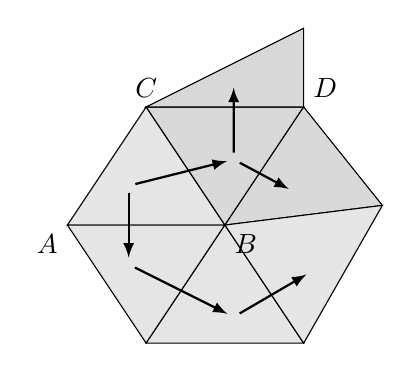
\begin{tikzpicture}
    % Define the vertices of the triangles
    \coordinate (A) at (0,0);
    \coordinate (B) at (2,0);
    \coordinate (C) at (1,1.5);
    \coordinate (D) at (3,1.5); % Extra vertex for the second triangle
    \coordinate (E) at (3,2.5); % Extra vertex for the second triangle
    \coordinate (F) at (4,0.25); % Extra vertex for the second triangle
    \coordinate (X) at (1,-1.5);
    \coordinate (Y) at (3,-1.5); % Extra vertex for the second triangle
    
    \coordinate (CentroidABC) at ($(A)!0.3333!(B)!0.3333!(C)$);
    \coordinate (CentroidBCD) at ($(B)!0.3333!(C)!0.3333!(D)$);
    \coordinate (CentroidCDE) at ($(C)!0.3333!(D)!0.3333!(E)$);
    \coordinate (CentroidBDF) at ($(B)!0.3333!(D)!0.3333!(F)$);
    \coordinate (CentroidABX) at ($(A)!0.3333!(B)!0.3333!(X)$);
    \coordinate (CentroidBXY) at ($(Y)!0.3333!(B)!0.3333!(X)$);
    \coordinate (CentroidBFY) at ($(Y)!0.3333!(B)!0.3333!(F)$);
    
    % Draw triangles
    \draw[fill=gray!20] (A) -- (B) -- (C) -- cycle; 
    \draw[fill=gray!30] (B) -- (C) -- (D) -- cycle; 
    \draw[fill=gray!30] (C) -- (D) -- (E) -- cycle; 
    \draw[fill=gray!30] (B) -- (D) -- (F) -- cycle; 
    \draw[fill=gray!20] (A) -- (B) -- (X) -- cycle; 
    \draw[fill=gray!20] (Y) -- (B) -- (X) -- cycle; 
    \draw[fill=gray!20] (Y) -- (B) -- (F) -- cycle; 
    
    % Draw arrows between triangle centroids
    \draw[-latex, thick, shorten <=2.5pt, shorten >=2.5pt] (CentroidABC) -- (CentroidBCD); 
    \draw[-latex, thick, shorten <=2.5pt, shorten >=2.5pt] (CentroidBCD) -- (CentroidCDE); 
    \draw[-latex, thick, shorten <=2.5pt, shorten >=2.5pt] (CentroidBCD) -- (CentroidBDF); 
    \draw[-latex, thick, shorten <=2.5pt, shorten >=2.5pt] (CentroidABC) -- (CentroidABX); 
    \draw[-latex, thick, shorten <=2.5pt, shorten >=2.5pt] (CentroidABX) -- (CentroidBXY); 
    \draw[-latex, thick, shorten <=2.5pt, shorten >=2.5pt] (CentroidBXY) -- (CentroidBFY); 
    
    % Labels for vertices (optional)
    \node at (A) [below left] {$A$};
    \node at (B) [below right] {$B$};
    \node at (C) [above] {$C$};
    \node at (D) [above right] {$D$};
\end{tikzpicture}
\caption{Strongly connected triangulation of a domain. The arrows depict a tree in the strong connection graph of the form used in Theorem~\ref{theorem:poincarefriedrichsestimate:grad}.}
\end{figure}

\begin{theorem}\label{theorem:poincarefriedrichsestimate:grad}
    \color{red}Precise form of the inequality yet to be discussed, though the construction principle is clear.
\end{theorem}

\begin{proof}
 Let $u \in W^{1,p}(\Omega)$. 
 For each $F \in \calT$ of dimension $n-1$, 
 we let $u_F \in W^{1,p}(U_F)$ such that $\nabla u_F = \nabla u$ over $U_F$ and such that $\| u_F \|_{L^{p}(U_F)} \leq C_{{\rm{P}},F} \| \nabla u_F \|_{L^{p}(U_F)}$.
 
 Since $\calT$ is strongly connected, there exists an enumeration of $n$-simplices $T_0, T_1, \dots, T_M$ such that for any $1 \leq m \leq M$ there exists some fixed but arbitrary $0 \leq j(m) < m$ such that $F_m := T_m \cap T_{j(m)}$ is a face of dimension $n-1$. We write $\Omega_m := \cup_{j=0}^{m} T_m$. Hence $\Omega = \Omega_M$. 
 
 
%  We let $T \in \calT$ be the first $n$-simplex. 
%  There exists We already have 
 
 Suppose that $1 \leq m \leq M$ such that there exists $w_{m-1} \in W^{1,p}(\Omega_{m-1})$ with $\nabla w_{m-1} = \nabla u$ over $\Omega_m$. Hence $c_{\star} := w_{m-1} - u_{|\Omega_{m-1}}$ is a constant. 
 By assumption, $T_{m}$ shares the face $F_{m}$ with $T_{j(m)}$. 
 Since $\nabla u_{F_{m}|T_{j(m)}} = \nabla w_{m-1|T_{j(m)}}$,
 there exists a constant $c_{m} := w_{m-1|T_{j(m)}} - u_{F_{m}|T_{j(m)}}$.
 We define $u'_{F_m} := u_{F_m} + c_{m} \in W^{1,p}(U_F)$.
 By construction, $\nabla u'_{F_m} = \nabla u_{F_m} = \nabla u_{|U_{F_m}}$ and $u_{F_{m}|T_{j(m)}} = w_{m-1|T_{j(m)}}$. 
 But that already implies $u'_{F_m} = u_{|F_m} - c_{\star}$. 
 As we define a measurable function $u'_{\star} \in W^{1,p}(\Omega_m)$ by extending $w_{m-1}$ with $u'_{F_m|T_m}$.
 Moreover, 
 \begin{gather*}
    \| u'_{F_m} \|_{L^{p}(T_m)}
    \leq 
    \| u_{F_m} \|_{L^{p}(T_m)}
    +
    \| c_{m} \|_{L^{p}(T_m)},
    \qquad 
    \| c_{m} \|_{L^{p}(T_m)}
    \leq 
    \frac{ \vol(T_m)^{\frac 1 p} }{ \vol(T_{j(m)})^{\frac 1 p} }
    \| c_{m} \|_{L^{p}(T_{j(m)})},
    \\ 
    \| c_{m} \|_{L^{p}(T_{j(m)})}
    \leq 
    \| w_{m-1}\|_{L^{p}(T_{j(m)})} + \| u_{F_{m}} \|_{L^{p}(T_{j(m)})} 
    .
 \end{gather*}
 In particular,
 \begin{align*}
    \| w_{m} \|_{L^{p}(T_m)}
    \leq 
    \| u_{F_m} \|_{L^{p}(T_m)}
    +
    \frac{ \vol(T_m)^{\frac 1 p} }{ \vol(T_{j(m)})^{\frac 1 p} }
    \| u_{F_{m}} \|_{L^{p}(T_{j(m)})}
    +
    \frac{ \vol(T_m)^{\frac 1 p} }{ \vol(T_{j(m)})^{\frac 1 p} }
    \| w_{m-1}\|_{L^{p}(T_{j(m)})}
    .
 \end{align*}
 We want to summarize the two integrals of $u_{F_m}$. 
 In the special case $p=1$,
 \begin{align*}
    \| w_{m} \|_{L^{1}(T_m)}
    \leq 
    \max\left(
        1, \frac{ \vol(T_m) }{ \vol(T_{j(m)}) } 
    \right)
    \| u_{F_m} \|_{L^{1}(U_{F_m})}
    +
    \frac{ \vol(T_m) }{ \vol(T_{j(m)}) }
    \| w_{m-1}\|_{L^{1}(T_{j(m)})}
    .
 \end{align*}
 In the special case $p=\infty$, 
 \begin{align*}
    \| w_{m} \|_{L^{\infty}(T_m)}
    \leq 
    2
    \| u_{F_m} \|_{L^{\infty}(U_{F_m})}
    +
    \| w_{m-1}\|_{L^{\infty}(T_{j(m)})}
    .
 \end{align*}
 When $1 < p < \infty$, letting $q$ be the complementary exponent, we observe 
 \begin{align*}
    \| w_{m} \|_{L^{p}(T_m)}
    &\leq 
    \left( 1 + \frac{ \vol(T_m)^{\frac q p} }{ \vol(T_{j(m)})^{\frac q p} } \right)^{\frac 1 q}
    \left( 
        \| u_{F_m} \|_{L^{p}(T_m)}^{p}
        +
        \| u_{F_{m}} \|_{L^{p}(T_{j(m)})}^{p}
    \right)^{\frac 1 p}
    +
    \frac{ \vol(T_m)^{\frac 1 p} }{ \vol(T_{j(m)})^{\frac 1 p} }
    \| w_{m-1}\|_{L^{p}(T_{j(m)})}
    \\&\leq 
    \left( 1 + \frac{ \vol(T_m)^{\frac q p} }{ \vol(T_{j(m)})^{\frac q p} } \right)^{\frac 1 q}
    \| u_{F_m} \|_{L^{p}(U_{F_m})} 
    +
    \frac{ \vol(T_m)^{\frac 1 p} }{ \vol(T_{j(m)})^{\frac 1 p} }
    \| w_{m-1}\|_{L^{p}(T_{j(m)})}
    .
 \end{align*}
 Recursive application provides the following estimate:
 if $T_0 = S_0, S_1, \dots, S_m = T_m$ is a sequence of $n$-simplices in $\calT$
 such that \color{red}$S_{t-1}$ precedes $S_{t}$ in the graph \color{black} and such that $F_t = S_t \cap S_{t-1}$,
 then 
 \begin{align*}
    \| w_{m} \|_{L^{p}(T_m)}
    &\leq 
    \sum_{t=1}^{m} 
    \left( 
        \prod_{t < l \leq m} 
        \frac{ \vol(T_l)^{\frac 1 p} }{ \vol(T_{l-1})^{\frac 1 p} } 
    \right)
    \left( 1 + \frac{ \vol(T_t)^{\frac q p} }{ \vol(T_{t-1})^{\frac q p} } \right)^{\frac 1 q}
    \| u_{F_t} \|_{L^{p}(U_{F_t})}
    \\&\quad \quad \quad 
    +
    \left( 
        \prod_{0 < l \leq m} 
        \frac{ \vol(T_l)^{\frac 1 p} }{ \vol(T_{l-1})^{\frac 1 p} } 
    \right)
    \| u_{T_0}\|_{L^{p}(T_{0})}
    .
 \end{align*}
 %  
 % \color{red}We want to summarize the Lp norms so that the Poincare inequality over $U_F$ is applied only once. In the special cases $p=1$ and $p=\infty$, this works as above. Do we have a formula for general $p$ that contains these as limit cases? \color{black}
 % In the special case $p < \infty$, we use the finite-dimensional H\"older inequality to find 
 % \begin{align*}
 %    \| w_{m} \|_{L^{p}(T_m)}^{p}
 %    &\leq 
 %    3^{p-1}
 %    \| u_{F_m} \|_{L^{p}(T_m)}^{p}
 %    +
 %    3^{p-1}
 %    \frac{ \vol(T_m) }{ \vol(T_{j(m)}) }
 %    \| u_{F_{m}} \|_{L^{p}(T_{j(m)})}^{p}
 %    +
 %    3^{p-1}
 %    \frac{ \vol(T_m) }{ \vol(T_{j(m)}) }
 %    \| w_{m-1}\|_{L^{p}(T_{j(m)})}^{p}
 %    \\&\leq 
 %    3^{p-1}
 %    \max\left( 1, \frac{ \vol(T_m) }{ \vol(T_{j(m)}) } \right)
 %    \| u_{F_m} \|_{L^{p}(U_{F_m})}^{p}
 %    +
 %    3^{p-1}
 %    \frac{ \vol(T_m) }{ \vol(T_{j(m)}) }
 %    \| w_{m-1}\|_{L^{p}(T_{j(m)})}^{p}
 %    ,
 % \end{align*}
 % and therefore
 % \begin{align*}
 %    \| w_{m} \|_{L^{p}(T_m)}
 %    &\leq 
 %    3^{\frac{p-1}{p}}
 %    \max\left( 1, \frac{ \vol(T_m) }{ \vol(T_{j(m)}) } \right)^{\frac 1 p}
 %    \| u_{F_m} \|_{L^{p}(U_{F_m})} 
 %    +
 %    3^{\frac{p-1}{p}}
 %    \frac{ \vol(T_m)^{\frac 1 p} }{ \vol(T_{j(m)})^{\frac 1 p} }
 %    \| w_{m-1}\|_{L^{p}(T_{j(m)})} 
 %    .
 % \end{align*}
 % \color{blue}
 % In the special case $p < \infty$, we use the finite-dimensional H\"older inequality to find 
 % \begin{align*}
 %    \| w_{m} \|_{L^{p}(T_m)}^{p}
 %    &\leq 
 %    \left( 
 %        1 + 2 \frac{ \vol(T_m)^{\frac{1}{p-1}} }{ \vol(T_{j(m)})^{\frac{1}{p-1}} }
 %    \right)^{ p-1 }
 %    \left( 
 %        \| u_{F_m} \|_{L^{p}(T_m)}^{p}
 %        +
 %        \| u_{F_{m}} \|_{L^{p}(T_{j(m)})}^{p}
 %        +
 %        \| w_{m-1}\|_{L^{p}(T_{j(m)})}^{p}
 %    \right)
 %    ,
 % \end{align*}
 % and therefore
 % \begin{align*}
 %    \| w_{m} \|_{L^{p}(T_m)}
 %    &\leq 
 %    \left( 
 %        1 + 2 \frac{ \vol(T_m)^{\frac{1}{p-1}} }{ \vol(T_{j(m)})^{\frac{1}{p-1}} }
 %    \right)^{ \frac{p-1}{p} }
 %    \left( 
 %        \| u_{F_m} \|_{L^{p}(T_m)} 
 %        +
 %        \| u_{F_{m}} \|_{L^{p}(T_{j(m)})} 
 %        +
 %        \| w_{m-1}\|_{L^{p}(T_{j(m)})} 
 %    \right)
 %    .
 % \end{align*}
 % \color{black}
\end{proof}

\begin{remark}
    The previous result depends on only a few parameters of the triangulation:
    the length of any traversal from the root simplex,
    the ratios of the volumes of adjacent simplices,
    the Poincar\'e constants on each face patch, and the Poincar\'e constant of the initial simplex. 
    The aforementioned local Poincar\'e constants can generally be estimated in terms of shape-parameters. 
    If the face patches of the triangulation are convex, then better estimates are possible. 
\end{remark}

% https://people.tamu.edu/~guermond//PUBLICATIONS/ern_guermond_m2an_2016.pdf 
% Lemma 5.5



\newpage

\section{Shellable triangulated domains}

% 2. Develop manifold-like complexes and characterize them 
We call an $n$-dimensional simplicial complex $\calT$ \emph{non-branching} if every $F \in \calT$ of dimension $n-1$ is contained in at most two $n$-simplices of $\calT$. We call those $F \in \calT$ of dimension $n-1$ contained within only one parent a \emph{boundary face}.
We write $\partial\calT$ for the simplicial subcomplex of $\calT$ of dimension $n-1$ 
whose full-dimensional members are exactly the boundary faces of $\calT$.

An $n$-dimensional simplicial complex is called \emph{manifold-like} if for every $x \in \bigcup \calT$
we have one of the following two conditions:
\begin{itemize}
 \item 
 there exists $\epsilon > 0$ 
 and a homeomorphism 
 \begin{align*}
    \phi : \Ball_\epsilon(x) \cap \bigcup\calT  
    \rightarrow 
    \left\{ x \in \bbR^{n} \suchthat |x| \leq 1 \right\}
 \end{align*}
 such that $\phi(x) = 0$,
 \item 
 there exists $\epsilon > 0$ and a homeomorphism 
 \begin{align*}
    \phi : \Ball_\epsilon(x) \cap \bigcup\calT 
    \rightarrow 
    \left\{ x \in \bbR^{n} \suchthat |x| \leq 1, x_n \leq 0 \right\}
 \end{align*}
 such that $\phi(x) = 0$.
\end{itemize}
This characterizes the union of the simplicial complex $\calT$ as a topological manifold with boundary. 

We would like to have a purely combinatorial and computable criterion that characterizes manifold-like simplicial complexes. A first step in that direction is the following result.

\begin{lemma}\label{lemma:characterizationofmanifoldcomplexes}
    Let $\calT$ be an $n$-dimensional simplicial complex. The following are equivalent:
    \begin{itemize}
     \item $\calT$ is manifold-like
     \item $\patch_{\calT}(V)$ is the triangulation of a ball for all $V \in \Vertices(\calT)$
     \item $\patch_{\calT}(V)$ is manifold-like for all $V \in \Vertices(\calT)$
     \item $\patch_{\calT}(S)$ is the triangulation of a ball for all $S \in \calT$
     \item $\patch_{\calT}(S)$ is manifold-like for all $S \in \calT$
    \end{itemize}
\end{lemma}
\begin{proof}
    \color{red} TODO
\end{proof}



\begin{remark}
    Clearly, not every simplicial complex is the triangulation of some (embedded) topological manifold with or without boundary. 
    Conversely, for each dimension $n \geq 5$ there exists an $n$-dimensional compact topological manifold without a triangulation. % TODO: are these compact?
    % TODO There are computational limits to algorithmically deciding whether a simplicial complex represents a manifold. 
\end{remark}



\begin{figure}
    \centering
    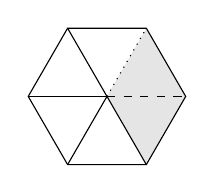
\begin{tikzpicture}
        \coordinate (O) at (0, 0);
        \coordinate (A) at ({cos(0)}, {sin(0)});
        \coordinate (B) at ({cos(60)}, {sin(60)});
        \coordinate (C) at ({cos(120)}, {sin(120)});
        \coordinate (D) at ({cos(180)}, {sin(180)});
        \coordinate (E) at ({cos(240)}, {sin(240)});
        \coordinate (F) at ({cos(300)}, {sin(300)});
        \fill[gray!20] (A) -- (B) -- (O) -- (F) -- cycle;
        \draw (A) -- (B) -- (C) -- (D) -- (E) -- (F) -- cycle;
        \draw[dashed] (O) -- (A); \draw[dotted] (O) -- (B); \draw (O) -- (C); \draw (O) -- (D); \draw (O) -- (E); \draw (O) -- (F);
    \end{tikzpicture}
    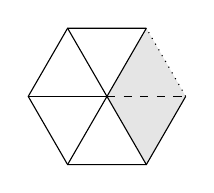
\begin{tikzpicture}
        \coordinate (O) at (0, 0);
        \coordinate (A) at ({cos(0)}, {sin(0)});
        \coordinate (B) at ({cos(60)}, {sin(60)});
        \coordinate (C) at ({cos(120)}, {sin(120)});
        \coordinate (D) at ({cos(180)}, {sin(180)});
        \coordinate (E) at ({cos(240)}, {sin(240)});
        \coordinate (F) at ({cos(300)}, {sin(300)});
        \fill[gray!20] (A) -- (B) -- (O) -- (F) -- cycle;
        \draw[dotted] (A) -- (B); \draw (B) -- (C) -- (D) -- (E) -- (F) -- (A);
        \draw[dashed] (O) -- (A); \draw (O) -- (B); \draw (O) -- (C); \draw (O) -- (D); \draw (O) -- (E); \draw (O) -- (F);
    \end{tikzpicture}
    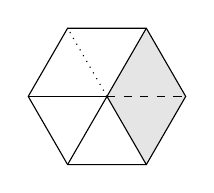
\begin{tikzpicture}
        \coordinate (O) at (0, 0);
        \coordinate (A) at ({cos(0)}, {sin(0)});
        \coordinate (B) at ({cos(60)}, {sin(60)});
        \coordinate (C) at ({cos(120)}, {sin(120)});
        \coordinate (D) at ({cos(180)}, {sin(180)});
        \coordinate (E) at ({cos(240)}, {sin(240)});
        \coordinate (F) at ({cos(300)}, {sin(300)});
        \fill[gray!20] (A) -- (B) -- (O) -- (F) -- cycle;
        \draw (A) -- (B) -- (C) -- (D) -- (E) -- (F) -- cycle;
        \draw[dashed] (O) -- (A); \draw (O) -- (B); \draw[dotted] (O) -- (C); \draw (O) -- (D); \draw (O) -- (E); \draw (O) -- (F);
    \end{tikzpicture}
    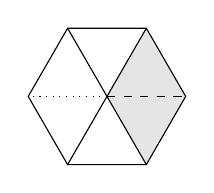
\begin{tikzpicture}
        \coordinate (O) at (0, 0);
        \coordinate (A) at ({cos(0)}, {sin(0)});
        \coordinate (B) at ({cos(60)}, {sin(60)});
        \coordinate (C) at ({cos(120)}, {sin(120)});
        \coordinate (D) at ({cos(180)}, {sin(180)});
        \coordinate (E) at ({cos(240)}, {sin(240)});
        \coordinate (F) at ({cos(300)}, {sin(300)});
        \fill[gray!20] (A) -- (B) -- (O) -- (F) -- cycle;
        \draw (A) -- (B) -- (C) -- (D) -- (E) -- (F) -- cycle;
        \draw[dashed] (O) -- (A); \draw (O) -- (B); \draw (O) -- (C); \draw[dotted] (O) -- (D); \draw (O) -- (E); \draw (O) -- (F);
    \end{tikzpicture}
    \caption{Examples and counterexamples for building a manifold-like $1$-patching of a $2$-dimensional manifold-like triangulation. (1) We have already added the edge patch along the dashed line and we add the edge patch along the dotted line. (2) The new edge patch may already be a subset of the subtriangulation (3) An inadmissible choice because new edge patch has no overlap with current subtriangulation, though the next subtriangulation would be manifold-like (4) An inadmissible choice because new edge patch has no overlap with current subtriangulation and the next subtriangulation would not be manifold-like.}\label{figure:illustrationpatching}
\end{figure}

\begin{figure}
    \centering
    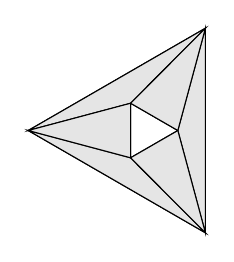
\begin{tikzpicture}[scale=0.5]
        \coordinate (O) at (0, 0);
        \coordinate (A) at ({0.8*cos(  0)}, {0.8*sin(  0)});
        \coordinate (B) at ({0.8*cos(120)}, {0.8*sin(120)});
        \coordinate (C) at ({0.8*cos(240)}, {0.8*sin(240)});
        \coordinate (X) at ({3.0*cos( 60)}, {3.0*sin( 60)});
        \coordinate (Y) at ({3.0*cos(180)}, {3.0*sin(180)});
        \coordinate (Z) at ({3.0*cos(300)}, {3.0*sin(300)});
        \draw (A) -- (B) -- (C) -- cycle; \draw (X) -- (Y) -- (Z) -- cycle;
        \draw[fill=gray!20] (X) -- (Y) -- (B) -- cycle;
        \draw[fill=gray!20] (Y) -- (Z) -- (C) -- cycle;
        \draw[fill=gray!20] (Z) -- (X) -- (A) -- cycle;
        \draw[fill=gray!20] (A) -- (X) -- (B) -- cycle;
        \draw[fill=gray!20] (B) -- (Y) -- (C) -- cycle;
        \draw[fill=gray!20] (C) -- (Z) -- (A) -- cycle;
    \end{tikzpicture}
    \begin{tikzpicture}[scale=0.5]
        \coordinate (O) at (0, 0);
        \coordinate (A) at ({3.0*cos(  0)}, {3.0*sin(  0)});
        \coordinate (B) at ({3.0*cos(120)}, {3.0*sin(120)});
        \coordinate (C) at ({3.0*cos(240)}, {3.0*sin(240)});
        \coordinate (X) at ({3.0*cos( 60)}, {3.0*sin( 60)});
        \coordinate (Y) at ({3.0*cos(180)}, {3.0*sin(180)});
        \coordinate (Z) at ({3.0*cos(300)}, {3.0*sin(300)});
        \draw (O) -- (A);
        \draw (O) -- (B);
        \draw (O) -- (C);
        \draw (O) -- (X);
        \draw (O) -- (Y);
        \draw (O) -- (Z);
        %
    \end{tikzpicture}
    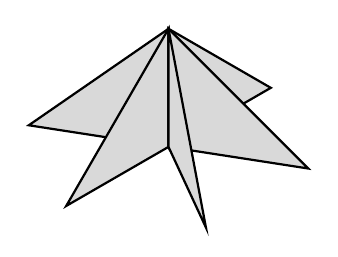
\begin{tikzpicture}[scale=0.5] 
        \tikzset{z={(90:1cm)}, y={(-30:1cm)}, x={(210:1cm)}}
        % \tikzset{z={(90:1cm)}, y={(-10:1cm)}, x={(250:1cm)}}

        \coordinate (O) at (0, 0);
        \coordinate (A) at ({3.0*cos(  0)}, {3.0*sin(  0)});
        \coordinate (B) at ({3.0*cos(120)}, {3.0*sin(120)});
        \coordinate (C) at ({3.0*cos(240)}, {3.0*sin(240)});
        \coordinate (X) at ({3.0*cos( 60)}, {3.0*sin( 60)});
        \coordinate (Y) at ({3.0*cos(180)}, {3.0*sin(180)});
        \coordinate (Z) at ({3.0*cos(300)}, {3.0*sin(300)});
        \coordinate (T) at ({0}, {0}, {3});

        \draw[thick, fill=gray!30] (O) -- (C) -- (T) -- cycle;
        \draw[thick, fill=gray!30] (O) -- (Y) -- (T) -- cycle;
        \draw[thick, fill=gray!30] (O) -- (Z) -- (T) -- cycle;
        \draw[thick, fill=gray!30] (O) -- (A) -- (T) -- cycle;
        \draw[thick, fill=gray!30] (O) -- (B) -- (T) -- cycle;
        \draw[thick, fill=gray!30] (O) -- (X) -- (T) -- cycle;
        
        
    \end{tikzpicture}

    \caption{Example of a connected $2$-dimensional manifold-like simplicial complex, which triangulates an annulus, that does neither admit a manifold-like $0$-patching nor manifold-like $1$-patching.}\label{figure:annuluscounterexample}
\end{figure}

% \color{red}
% \begin{proposition}
%     Suppose that $\calT$ is a connected $n$-dimensional simplicial complex. Then the following are equivalent:
%     \begin{itemize}
%      \item $\calT$ is manifold-like
%      \item $\calT$ has a manifold-like $0$-patching
%      % \item There exists $1 \leq k \leq n$ such that $\calT$ has a $k$-patching
%     \end{itemize}
% \end{proposition}
% \color{black}





% 3. Shellability 
\subsection{Shellable simplicial complexes}

We turn our attention to a different idea of how to incrementally construct a simplicial complex while maintaining well-behaved intermediate complexes. 
Given an $n$-dimensional simplicial complex $\calT$, a \emph{shelling} is an enumeration of the $n$-simplices $T_{0}, T_{1}, T_{2}, \dots \in \subsimplex_{n}(\calT)$ such that $( \patch_{\calT}(T_{0}) \cup \patch_{\calT}(T_{1}) \cup \dots \cup \patch_{\calT}(T_{m}) ) \cap \patch_{\calT}(T_{m+1})$ is a simplicial complex of dimension $n-1$. Notice that the last intersection is automatically a subcomplex of the boundary complex of the last simplex $T_{m}$, and is thus manifold like. 


% \begin{lemma}
%     If an $n$-dimensional simplicial complex $\calT$ has a shelling $T_{0}, T_{1}, T_{2}, \dots$, then it is manifold-like.
%     In particular, $\patch_{\calT}(T_{0}) \cup \patch_{\calT}(T_{1}) \cup \dots \cup \patch_{\calT}(T_{m})$ is manifold-like for every $m \geq 0$.
% \end{lemma}
% \begin{proof}    
% \end{proof}

We notion of shelling is taken from Ziegler's book~\cite{ziegler2012lectures}

% TODO: Ziegler, Lemma 8.7: if a complex has a shelling, then this gives a shelling of the stars 

% 

A simplicial $n$-dimensional complex $\calT$ is called shellable if its $n$-simplices can be arranged in linear order $T_0, T_1, \dots$ in such a way that the subcomplex $( \cup_{i=0}^{k-1} T_i ) \cap T_k$ has dimension $n-1$ for all $k > 0$.


\begin{remark}
    A shellable simplicial complex that triangulates a manifold has a very restricted topology. 
    The Mayer-Vietoris theorem implies restrictions on the homology groups of simplicial complexes iteratively constructed via shelling. 

    Suppose that $\calT$ is a strongly connected $n$-dimensional simplicial complex that triangulates a manifold, and suppose that its boundary complex $\partial\calT$ is either empty or strongly connected.  
    Suppose furthermore that $T$ is an $n$-simplex, $T \notin \calT$, whose boundary complex intersects with $\partial\calT$ at a non-empty simplicial complex $\calS$ of dimension $n-1$. In particular, $\calS$ is either the whole boundary complex of $T$ or a patch around a proper subsimplex of $T$. We write $\calT'$ be the  simplicial complex that contains $\calT \cup T$.
    We exclude that case $n \leq 1$ since otherwise the discussion is trivial.
    
    According to the simplicial Mayer-Vietoris theorem, there exists an exact sequence 
    \begin{align*}
        \begin{CD}
            \dots \longrightarrow H_{k}(\calS) \longrightarrow H_{k}(\calT \oplus T) \longrightarrow H_{k}(\calT') \longrightarrow H_{k-1}(\calS) \longrightarrow\dots 
        \end{CD}
    \end{align*}
    We notice that $\calS$, $\calT$, $T$ and $\calT'$ are each connected, and hence their zeroth homology groups are isomorphic to $\bbZ$. 
    By the nature of the mappings in the Mayer-Vietoris sequence, 
    \color{red}which uses some specific knowledge about the arrows\color{black}, 
    we see that 
    \begin{align*}
        \begin{CD}
            0 \longrightarrow H_{0}(\calS) \longrightarrow H_{0}(\calT) \oplus H_{0}(T) \longrightarrow H_{0}(\calT') \longrightarrow 0 
        \end{CD}
    \end{align*}
    is an exact sequence. 
    Moreover, $H_{k}(\calS) = H_{k}(T) 0$ for $0 < k < n-1$. Hence, for $1 < k < n-1$,
    the Mayer-Vietoris sequence includes the exact sequence 
    \begin{align*}
        \begin{CD}
            0 \longrightarrow H_{k}(\calT \oplus T) \longrightarrow H_{k}(\calT') \longrightarrow 0 
        \end{CD}
    \end{align*}
    and we conclude that $H_{k}(\calT) = 0$ for $0 < k < n-1$.
    Finally, the Mayer-Vietoris sequence includes the exact sequences 
    \begin{align*}
        \begin{CD}
            0 \longrightarrow H_{n}(\calT \oplus T) \longrightarrow H_{n}(\calT') \longrightarrow H_{n-1}(\calS) \longrightarrow H_{n-1}(\calT \oplus T) \longrightarrow H_{n-1}(\calT') \longrightarrow 0 
        \end{CD}
    \end{align*}
    % Here, if $n=1$, it already follows that $H_{n}(\calT \oplus T) \simeq H_{n}(\calT')$.
    % % We know that  $H_{0}(\calT') \simeq H_{0}(\calT) \simeq H_{0}(T) \simeq H_{0}(\calS) \simeq \bbZ$ because the respective simplicial complexes are path-connected. 
    % Hence $H_{1}(\calT) \oplus H_{1}(T) \simeq H_{1}(\calT')$. 
    % one easily sees that $H_{0}(\calT') \simeq \bbZ$ and $H_{1}(\calT) \oplus H_{1}(T) \simeq H_{1}(\calT')$. 
    Since $\calT$ and $T$ are triangulations of manifolds with non-empty boundary, their $n$-th simplicial homology groups vanish. 
    In the case that $\calS$ is isomorphic to disk,
    then $H_{n}(\calT') \simeq H_{n}(\calT \oplus T)$ are trivial and $H_{n-1}(\calT') \simeq H_{n-1}(\calT \oplus T)$ follows.
    Consider now the case that $\calS$ is isomorphic to a sphere.
    Since the boundary complex of $\calT$ is strongly connected and non-branching, it must coincide with $\calS$. Hence $\calT'$ triangulates a manifold without boundary, and thus $H_{n}(\calT') \simeq \bbZ$. 
    \color{red}By some handwaving argument, $H_{n}(\calT') \longrightarrow H_{n-1}(\calS)$ is an isomorphism.\color{black}
    Hence $H_{n-1}(\calT) \rightarrow H_{n-1}(\calT')$ is an isomorphism.
    
    We conclude that the simplicial homology groups of a shellable $n$-dimensional simplicial complex $\calT$ that triangulates a manifold satisfy 
    \[
        H_0(\calT) \simeq \bbZ, 
        \quad 
        H_1(\calT) \simeq \dots \simeq H_{n-1}(\calT) \simeq 0.
    \]
    Moreover, $H_n(\calT) \simeq \bbZ$ if $\calT$ has no boundary and $H_n(\calT) \simeq 0$ otherwise. 
    
    % then $H_{n}(\calT') \simeq H_{n}(\calT \oplus T)$ and $H_{n-1}(\calT') \simeq H_{n-1}(\calT \oplus T)$ follow immediately.
    % Moreover, Thus $H_{n}(\calT') = H_{n}(\calT) \oplus H_{n}(\calS)$.
    % We conclude that any shellable simplicial complex has the homology groups of a disk or a sphere. 
    % NB: the zeroth homology is always free, and the n-th homology group, being the kernel of a mapping free abelian group, is free as well.
    % \begin{align*}
    %     \begin{CD}
    %         0 \longrightarrow H_{1}(\calT) \oplus H_{1}(T) \longrightarrow H_{1}(\calT') \longrightarrow H_{0}(\calS) \longrightarrow H_{0}(\calT) \oplus H_{0}(T) \longrightarrow H_{0}(\calT') \longrightarrow 0 
    %     \end{CD}
    % \end{align*}
\end{remark}


\section{Constructive estimate of Poincar\'e--Friedrichs constants}
% Repeat for H(curl), H(div), and differential forms 

\section*{Acknowledgments}

\bibliographystyle{plain}
\bibliography{library}

\end{document}
